\documentclass[border=10pt]{standalone}
\usepackage{tikz}
\usetikzlibrary{arrows.meta,positioning,shapes.geometric,fit,calc,backgrounds}

\begin{document}
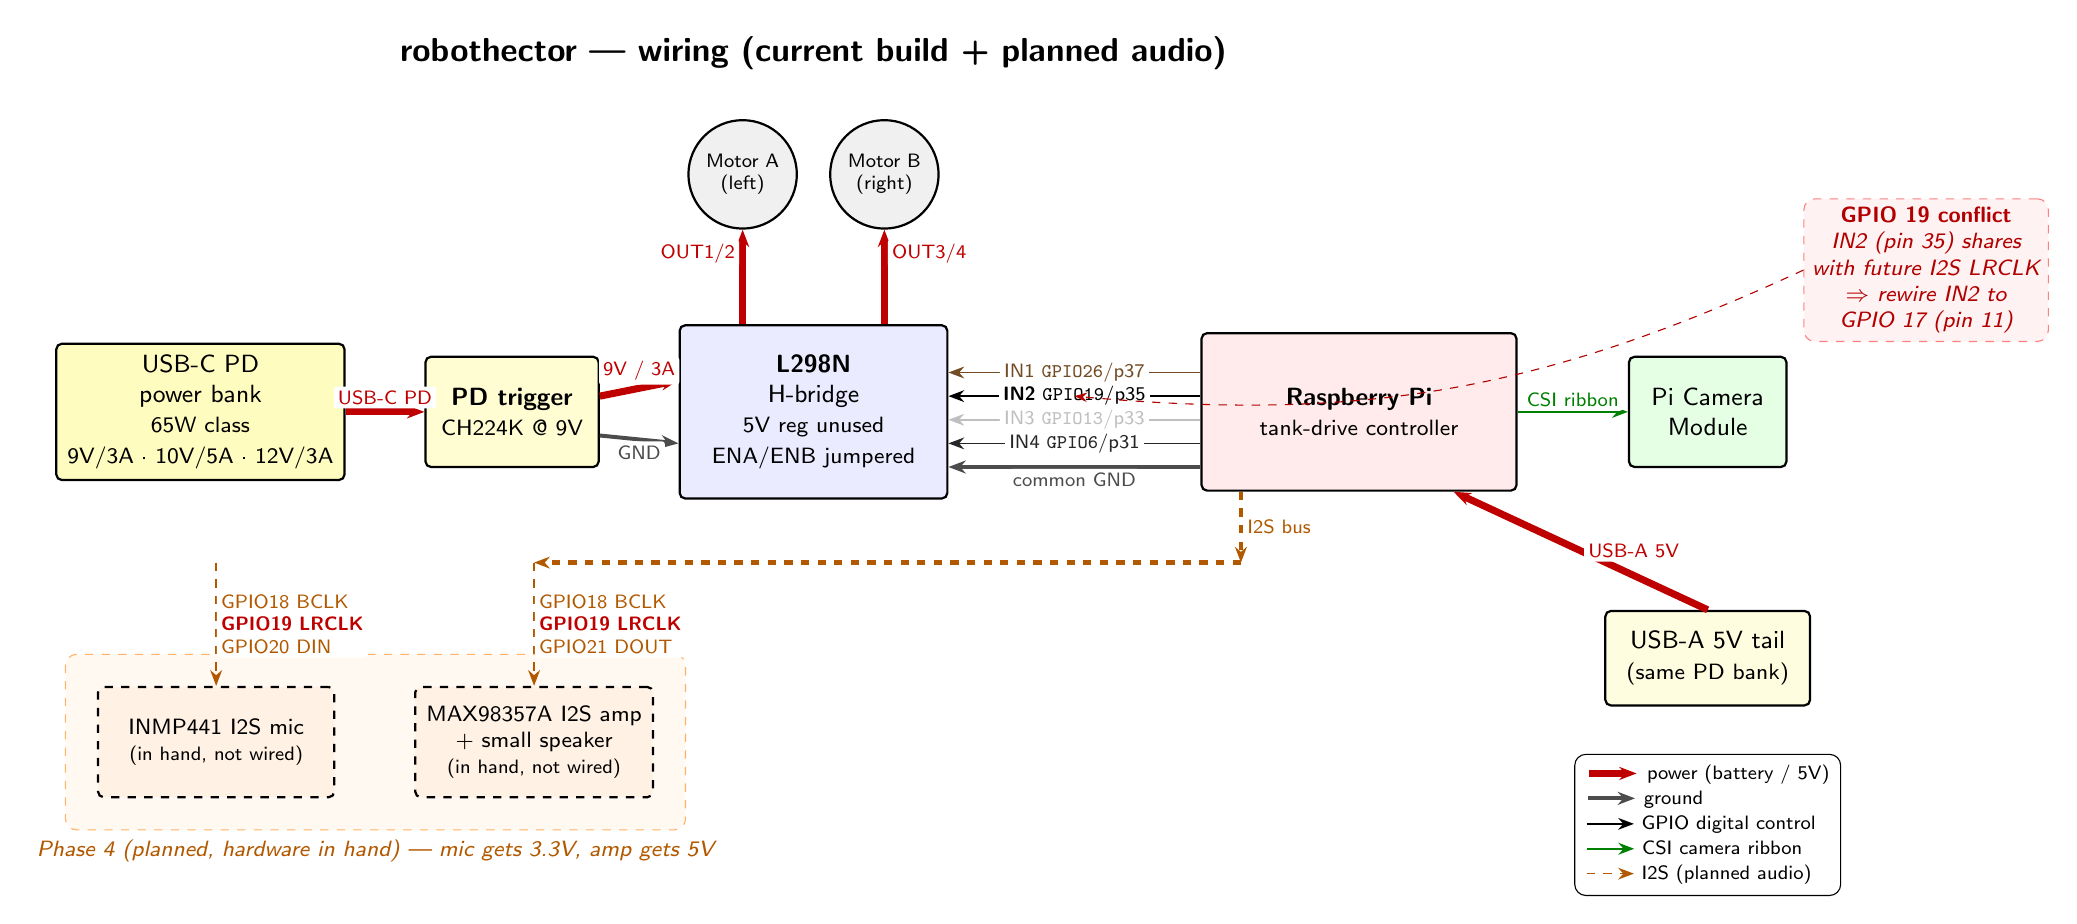
\begin{tikzpicture}[
    font=\sffamily\small,
    block/.style    ={draw, thick, rounded corners=2pt, align=center,
                      minimum height=10mm, inner sep=4pt, fill=white},
    pi/.style       ={block, fill=red!8,    minimum width=40mm, minimum height=20mm},
    bridge/.style   ={block, fill=blue!8,   minimum width=34mm, minimum height=22mm},
    batt/.style     ={block, fill=yellow!25, minimum width=24mm, minimum height=14mm},
    usb/.style      ={block, fill=yellow!12, minimum width=26mm, minimum height=12mm},
    motor/.style    ={draw, thick, circle, minimum size=13mm, fill=gray!12,
                      align=center, font=\sffamily\scriptsize},
    cam/.style      ={block, fill=green!10, minimum width=20mm, minimum height=14mm},
    audio/.style    ={block, dashed, fill=orange!10, minimum width=30mm,
                      minimum height=14mm, font=\sffamily\footnotesize, align=center},
    pwr/.style      ={-{Stealth[length=2.2mm]}, line width=0.9mm, red!75!black},
    gnd/.style      ={-{Stealth[length=2.2mm]}, line width=0.5mm, black!70},
    ctrl/.style     ={-{Stealth[length=2mm]}, semithick},
    i2s/.style      ={-{Stealth[length=2mm]}, semithick, dashed, orange!70!black},
    csi/.style      ={-{Stealth[length=2mm]}, thick, green!50!black},
    wlbl/.style     ={font=\sffamily\scriptsize, inner sep=1.5pt, fill=white,
                      rounded corners=1pt},
    note/.style     ={font=\sffamily\footnotesize\itshape, align=center,
                      text=black!60},
  ]

  % ============ MAIN HORIZONTAL ROW ============
  \node[batt] (batt) {USB-C PD\\power bank\\\footnotesize 65W class\\\footnotesize 9V/3A · 10V/5A · 12V/3A};
  \node[block, fill=yellow!18, right=10mm of batt, minimum width=22mm,
        minimum height=14mm, align=center] (pdtrig)
        {\textbf{PD trigger}\\\footnotesize CH224K @ 9V};
  \node[bridge, right=10mm of pdtrig] (l298)
        {\textbf{L298N}\\H-bridge\\\footnotesize 5V reg unused\\\footnotesize ENA/ENB jumpered};
  \node[pi, right=32mm of l298] (pi)
        {\textbf{Raspberry Pi}\\\footnotesize tank-drive controller};
  \node[cam, right=14mm of pi] (cam) {Pi Camera\\Module};

  % motors above L298N (chassis-mounted)
  \node[motor, above=12mm of l298, xshift=-9mm] (mA) {Motor A\\(left)};
  \node[motor, above=12mm of l298, xshift= 9mm] (mB) {Motor B\\(right)};

  % USB-A 5V tail from the same bank, routed below to feed Pi
  \node[usb, below=18mm of cam] (usb) {USB-A 5V tail\\\footnotesize(same PD bank)};

  % Audio modules: bottom-LEFT, below batt + L298N
  \node[audio, below=26mm of batt, xshift=2mm] (mic)
        {INMP441 I2S mic\\\scriptsize(in hand, not wired)};
  \node[audio, right=10mm of mic] (amp)
        {MAX98357A I2S amp\\+ small speaker\\\scriptsize(in hand, not wired)};

  % ============ POWER ============
  % bank → PD trigger (USB-C, PD negotiates 9V)
  \draw[pwr] (batt.east) -- node[wlbl, above]{USB-C PD} (pdtrig.west);
  % PD trigger → L298N V+ (regulated 9V up to 3A)
  \draw[pwr] ([yshift= 2mm]pdtrig.east)
        -- node[wlbl, above]{9V / 3A} ([yshift= 4mm]l298.west);
  \draw[gnd] ([yshift=-3mm]pdtrig.east)
        -- node[wlbl, below]{GND}     ([yshift=-4mm]l298.west);

  % USB-A 5V tail (same bank, different port) → Pi
  \draw[pwr] (usb.north) -- node[wlbl, right]{USB-A 5V}
             ([xshift=12mm]pi.south);

  % L298N → motors
  \draw[pwr] ([xshift=-9mm]l298.north) -- node[wlbl, near end, left]{OUT1/2} (mA.south);
  \draw[pwr] ([xshift= 9mm]l298.north) -- node[wlbl, near end, right]{OUT3/4} (mB.south);

  % common GND between Pi and L298N
  \draw[gnd] ([yshift=-7mm]pi.west) -- node[wlbl, below]{common GND}
             ([yshift=-7mm]l298.east);

  % ============ CONTROL Pi → L298N (4 wires) ============
  \draw[ctrl, brown!60!black]
        ([yshift= 5mm]pi.west) -- ([yshift= 5mm]l298.east)
        node[wlbl, pos=0.5]{IN1 \texttt{GPIO26}/p37};
  \draw[ctrl, black]
        ([yshift= 2mm]pi.west) -- ([yshift= 2mm]l298.east)
        node[wlbl, pos=0.5]{\textbf{IN2} \texttt{GPIO19}/p35};
  \draw[ctrl, gray!50]
        ([yshift=-1mm]pi.west) -- ([yshift=-1mm]l298.east)
        node[wlbl, pos=0.5]{IN3 \texttt{GPIO13}/p33};
  \draw[ctrl, gray!30!black]
        ([yshift=-4mm]pi.west) -- ([yshift=-4mm]l298.east)
        node[wlbl, pos=0.5]{IN4 \texttt{GPIO6}/p31};

  % GPIO 19 conflict callout (top-right corner, points at IN2 wire)
  \coordinate (in2mid) at ($(pi.west)!0.5!(l298.east) + (0,2mm)$);
  \node[note, text=red!70!black, align=center,
        draw=red!50, dashed, rounded corners, fill=red!5, inner sep=3pt,
        right=2mm of cam, anchor=west,
        yshift=18mm]
       (conflict) {\textbf{GPIO 19 conflict}\\IN2 (pin 35) shares\\with future I2S LRCLK\\
                   $\Rightarrow$ rewire IN2 to\\GPIO 17 (pin 11)};
  \draw[red!70!black, dashed, -{Stealth[length=1.6mm]}]
        (conflict.west) to[bend left=15] (in2mid);

  % ============ CSI ============
  \draw[csi] (pi.east) -- node[wlbl, above]{CSI ribbon} (cam.west);

  % ============ I2S (future) — single bus from Pi, splits to mic + amp ============
  % bus stub from Pi.south-west, drops then runs left along a backbone above audio
  \coordinate (i2sStub) at ([xshift=-15mm]pi.south);
  \coordinate (i2sBus)  at ($(i2sStub)+(0,-9mm)$);
  \coordinate (busOverMic) at (mic.north |- i2sBus);
  \coordinate (busOverAmp) at (amp.north |- i2sBus);

  % vertical drop from Pi.south + horizontal backbone to above each module
  \draw[i2s, line width=0.6mm] (i2sStub) -- (i2sBus)
        node[wlbl, pos=0.5, right]{\scriptsize I2S bus};
  \draw[i2s, line width=0.6mm] (i2sBus) -- (busOverAmp);

  % branch down to mic
  \draw[i2s] (busOverMic) -- (mic.north)
        node[wlbl, pos=0.5, right, align=left]
            {\scriptsize GPIO18 BCLK\\
             \scriptsize {\color{red!75!black}\textbf{GPIO19 LRCLK}}\\
             \scriptsize GPIO20 DIN};

  % branch down to amp
  \draw[i2s] (busOverAmp) -- (amp.north)
        node[wlbl, pos=0.5, right, align=left]
            {\scriptsize GPIO18 BCLK\\
             \scriptsize {\color{red!75!black}\textbf{GPIO19 LRCLK}}\\
             \scriptsize GPIO21 DOUT};

  % ============ Phase 4 group box ============
  \begin{scope}[on background layer]
    \node[draw=orange!60, dashed, rounded corners, fill=orange!5,
          fit=(mic)(amp), inner sep=4mm] (audiogrp) {};
  \end{scope}
  \node[font=\sffamily\footnotesize\itshape, text=orange!70!black,
        anchor=north] at (audiogrp.south)
        {Phase 4 (planned, hardware in hand) --- mic gets 3.3V, amp gets 5V};

  % ============ TITLE ============
  \node[font=\sffamily\large\bfseries, anchor=south, align=center]
        at ($(mA)!0.5!(mB) + (0,12mm)$)
        {robothector --- wiring (current build + planned audio)};

  % ============ LEGEND (bottom-right, away from everything) ============
  \node[draw, rounded corners, fill=white, inner sep=4pt,
        anchor=north, align=left,
        font=\sffamily\scriptsize] (legend)
        at ([yshift=-6mm]usb.south)
        {\tikz{\draw[pwr]  (0,0)--(6mm,0);}\ power (battery / 5V)\\[1pt]
         \tikz{\draw[gnd]  (0,0)--(6mm,0);}\ ground\\[1pt]
         \tikz{\draw[ctrl] (0,0)--(6mm,0);}\ GPIO digital control\\[1pt]
         \tikz{\draw[csi]  (0,0)--(6mm,0);}\ CSI camera ribbon\\[1pt]
         \tikz{\draw[i2s]  (0,0)--(6mm,0);}\ I2S (planned audio)};

\end{tikzpicture}
\end{document}
